\techsection{FRONT VIEW}
\vspace{-0.3cm}

\begin{tabular}{p{0.49\textwidth}|p{0.49\textwidth}}
% Left side
\begin{center}
\begin{tikzpicture}
\node[draw=bordercolor, line width=1pt, inner sep=4pt, fill=white, rounded corners=2pt] {
    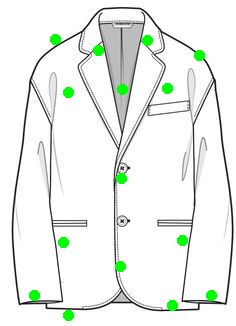
\includegraphics[width=0.35\textwidth,height=12cm,keepaspectratio]{blazer_illustration_front.png}% FRONT IMAGE
};
\end{tikzpicture}
\end{center}
&
% Right side - Attributes Table
\specificationtable{
1 & Lapel/collar connection. Maintain crisp shaping using structured interfacing. \\  
2 & Left lower side seam. Reinforce seam to handle daily wear. \\ 
3 & Left hem corner. Clean folded edge with even stitching. \\ 
4 & Right hem corner. Mirror left side construction with matching topstitch. \\ 
5 & Upper front button area. Ensure properly aligned buttonhole for neat closure. \\ 
6 & Lower front button area. Reinforce for extra security. \\ 
7 & Left hip pocket. Construct as a double welt pocket with reinforced edges. \\ 
8 & Right hip pocket. Mirror construction and placement of left pocket. \\ 
9 & Left shoulder seam. Integrate moderate shoulder padding for structure. \\ 
10 & Right shoulder seam. Match padding and seam allowance to left shoulder. \\ 
}
\end{tabular}

\vspace{0.5cm}

% MEASUREMENTS TABLE
\measurementtable{
Shoulder Width & 48\,cm & \pm1\,cm & Chest Circumference & 100\,cm & \pm2\,cm & \\ 
Waist Circumference & 92\,cm & \pm2\,cm & Front Length & 74\,cm & \pm1\,cm & \\ 
Sleeve Length & 61\,cm & \pm1\,cm & Lapel Width & 7\,cm & \pm0.5\,cm & \\ 
}

\techsection{BACK VIEW}
\vspace{-0.3cm}

\begin{tabular}{p{0.49\textwidth}|p{0.49\textwidth}}
% Left side
\begin{center}
\begin{tikzpicture}
\node[draw=bordercolor, line width=1pt, inner sep=4pt, fill=white, rounded corners=2pt] {
    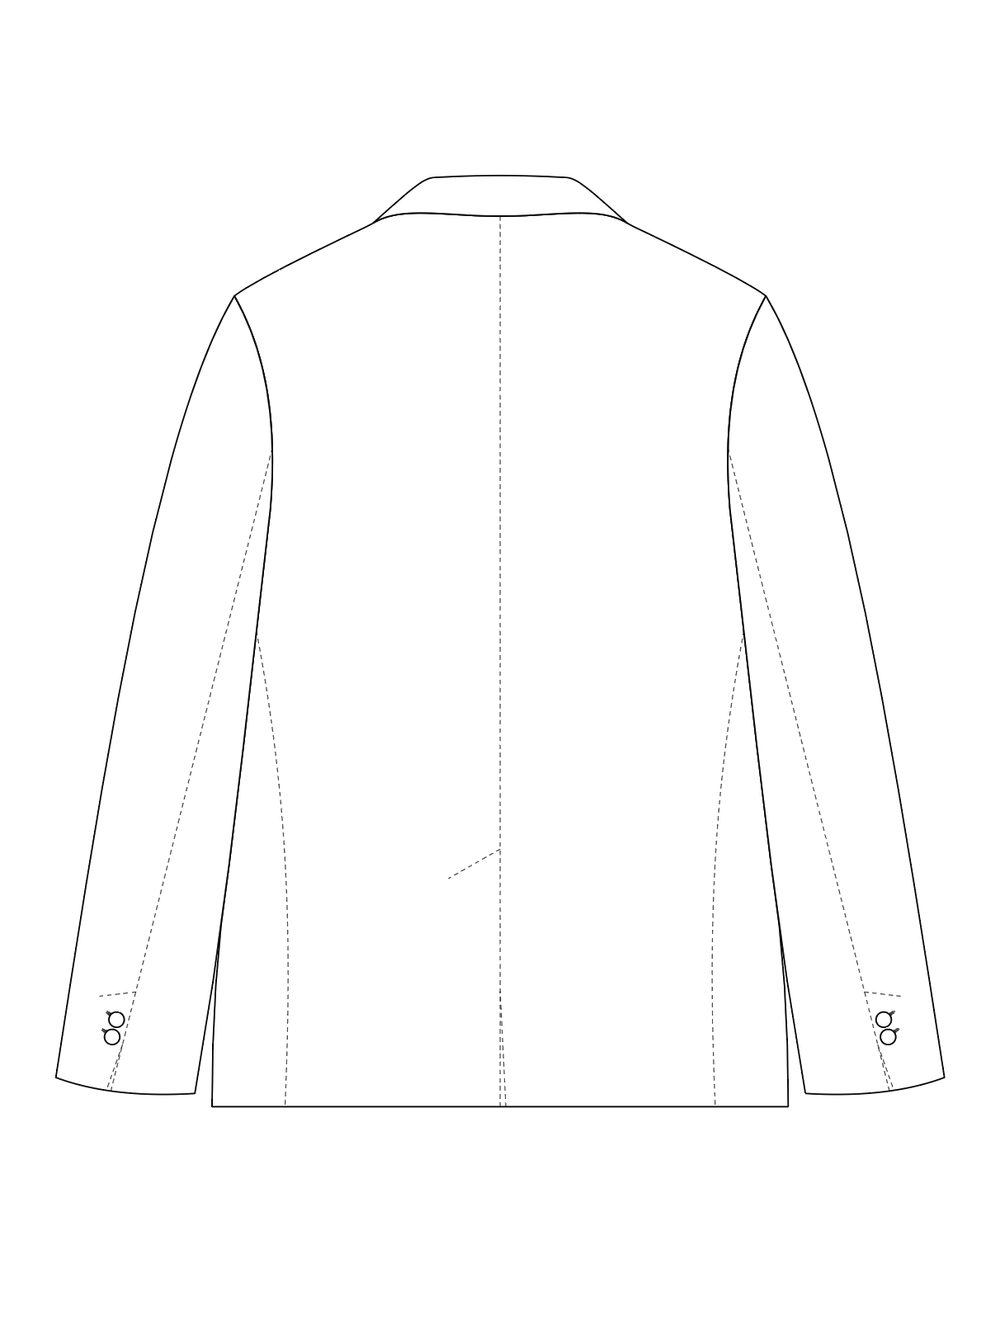
\includegraphics[width=0.35\textwidth,height=12cm,keepaspectratio]{blazer_illustration_back.png}% BACK IMAGE
};
\end{tikzpicture}
\end{center}
&
% Right side - Attributes Table
\specificationtable{
1 & Top collar join. Use stable interfacing at the collar seam. \\ 
2 & Right cuff end. Reinforce vent and cuff edge. \\ 
3 & Left cuff end. Mirror reinforcement and stitching from right cuff. \\ 
4 & Right waist area. Secure side seam with slight taper. \\ 
5 & Left waist area. Balance tension with right waist seam. \\ 
6 & Center back seam. Match pattern and ensure seam is pressed flat. \\ 
7 & Upper center back. Allow slight ease for comfortable fit across shoulders. \\ 
8 & Lower center back. Consider a vent or pleat for range of movement. \\ 
9 & Left side back panel. Maintain symmetrical shaping with right side. \\ 
10 & Right side back panel. Mirror fit and style lines from left side. \\ 
11 & Right upper shoulder. Reinforce shoulder seam with tape if needed. \\ 
12 & Left upper shoulder. Match construction details of right shoulder. \\ 
}
\end{tabular}

\vspace{0.5cm}

% MEASUREMENTS TABLE
\measurementtable{
Back Width & 47\,cm & \pm1\,cm & Center Back Length & 76\,cm & \pm1\,cm & \\ 
Sleeve Inseam & 44\,cm & \pm1\,cm & Armhole Depth & 23\,cm & \pm0.5\,cm & \\ 
Back Neck Width & 18\,cm & \pm0.5\,cm & Hem Width & 53\,cm & \pm1\,cm & \\ 
}
